Independence is what gives a differential oracle its authority. If the reference is
independent of the system under test, agreement is evidence and disagreement is a
defect. The word, however, is doing two jobs at once.

\subsection{Two questions, not one}

\emph{Implementation independence} answers: could the reference have inherited a
defect through shared \textbf{logic}? Shared code, a shared reading of the
specification, a shared author. This is the sense the literature grades. A recent
review of oracle sources orders exactly this axis, placing an independently
developed reference above a comparison among existing implementations, and that
above consensus among implementations drawn from one origin~\cite{oraclesurvey2026}.

\emph{Evidential independence} answers a different question: could the reference
inherit a defect through shared \textbf{evidence}? If the reference's inputs are
artifacts produced by the system under test, a defect in the producer propagates
into the reference's premises. The reference then computes correctly from corrupted
inputs and agrees with the system---for the same wrong reason.

The two are orthogonal, and this is what makes the second worth naming. An oracle
can hold maximal implementation independence and none of the evidential kind: a
reference written by different people, in a different language, from the
specification rather than from the code, which nonetheless takes the system's own
internal state as its input. Its logic shares nothing. Its premises share
everything. Figure~\ref{fig:axes} places both axes, and the techniques discussed in
Section~7 on them; the two corners that matter most are occupied by two oracles for
the same component.

\begin{figure}[t]
\centering
%% GATE: if the TikZ box exceeds the column width LaTeX does NOT WARN with an overfull hbox -- the box
%% silently spills over the neighboring column. We measure it and stop the build.
%% Measured (2026-09-11): box 210.7pt, \columnwidth 241.1pt.
\sbox0{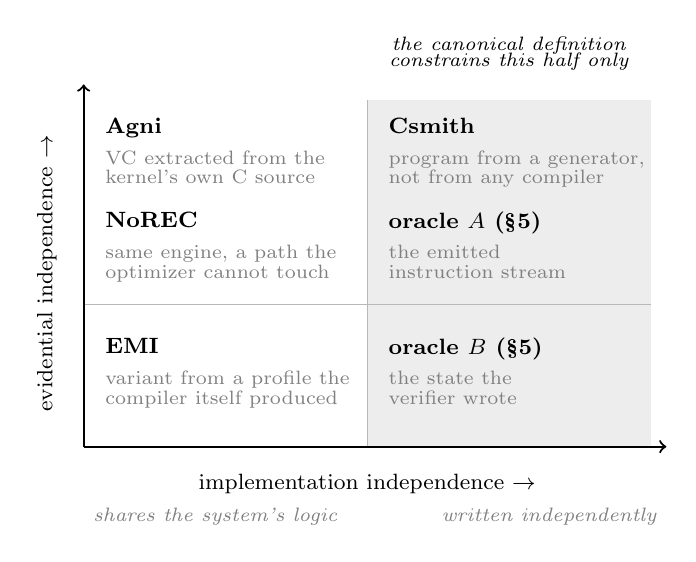
\begin{tikzpicture}[x=1mm,y=1mm,font=\footnotesize]
  \definecolor{gridgrey}{gray}{0.72}
  \definecolor{bandgrey}{gray}{0.93}
  %% Layout (B feedback): a column-filling width (76mm), a height cut in half
  %% (44mm), a font one size larger. Because the top half carries two entries
  %% (Agni, NoREC) it is taller than the bottom; the middle line is semantic, not a ratio.
  \fill[bandgrey] (36,0) rectangle (72,44);
  \draw[gridgrey] (0,18) -- (72,18);
  \draw[gridgrey] (36,0) -- (36,44);
  \draw[->,thick] (0,0) -- (74,0);
  \draw[->,thick] (0,0) -- (0,46);

  \node[anchor=north] at (36,-2.2) {implementation independence $\rightarrow$};
  \node[rotate=90,anchor=south] at (-2.2,22) {evidential independence $\rightarrow$};
  \node[anchor=north west,gray,font=\scriptsize\itshape] at (0,-6.5) {shares the system's logic};
  \node[anchor=north east,gray,font=\scriptsize\itshape] at (74,-6.5) {written independently};

  %% each entry is two nodes: a bold name + a gray two-line description
  \node[anchor=north west] at (1.5,43) {\textbf{Agni}};
  \node[anchor=north west,align=left,font=\scriptsize,text=gray] at (1.5,38.8) {VC extracted from the\\[-1pt]kernel's own C source};
  \node[anchor=north west] at (1.5,31) {\textbf{NoREC}};
  \node[anchor=north west,align=left,font=\scriptsize,text=gray] at (1.5,26.8) {same engine, a path the\\[-1pt]optimizer cannot touch};
  \node[anchor=north west] at (37.5,43) {\textbf{Csmith}};
  \node[anchor=north west,align=left,font=\scriptsize,text=gray] at (37.5,38.8) {program from a generator,\\[-1pt]not from any compiler};
  \node[anchor=north west] at (37.5,31) {\textbf{oracle $A$ (\S5)}};
  \node[anchor=north west,align=left,font=\scriptsize,text=gray] at (37.5,26.8) {the emitted\\[-1pt]instruction stream};
  \node[anchor=north west] at (1.5,15) {\textbf{EMI}};
  \node[anchor=north west,align=left,font=\scriptsize,text=gray] at (1.5,10.8) {variant from a profile the\\[-1pt]compiler itself produced};
  \node[anchor=north west] at (37.5,15) {\textbf{oracle $B$ (\S5)}};
  \node[anchor=north west,align=left,font=\scriptsize,text=gray] at (37.5,10.8) {the state the\\[-1pt]verifier wrote};
  \node[anchor=south,align=center,font=\scriptsize\itshape] at (54,46.5)
    {the canonical definition\\[-2pt]constrains this half only};
\end{tikzpicture}}%
\ifdim\wd0>\columnwidth
  \typeout{FIGWIDTH-ERROR box=\the\wd0 column=\the\columnwidth}%
\fi
\usebox0
\caption{The two axes, with the techniques of Section~7 placed on both. Height is
what an oracle reads: low means it reads what the system produced, high means it reads
something upstream of that. The shaded
half is what a pseudo-oracle is defined to be~\cite{barr2015oracle}: the condition
$f_1 \neq f_2$ fixes a horizontal position and says nothing about height. Agni and
oracle $B$ are mirror images---one encodes the component's own logic but reads its
source, upstream of every value it computes; the other is written independently but
reads what the component produced. Csmith occupies the corner it never claims: its
independence argument is made on the horizontal axis, while what protects it is its
height.}
\label{fig:axes}
\end{figure}


\subsection{The axis is component-relative}

Evidential independence is not a relation between an oracle and a system. It is a
relation between an oracle and the \textbf{component under test}, and an oracle may
share almost all of a system with the code it judges while remaining evidentially
independent of the part it is judging.

NoREC is the clean illustration~\cite{rigger2020norec}. Its reference is the same
database engine: same parser, same storage, same execution. What it changes is that
the query is rewritten into a form the optimizer cannot apply to. Relative to the
optimizer---the component under test---the reference's evidence does not pass
through the code being judged. Relative to the execution engine, it plainly does.

Read component-relatively, the axis predicts the shape of the limitation NoREC's
authors report, and they report it: ``both the unoptimized and optimized query can
yield an incorrect result''. Their framing is that metamorphic testing cannot
establish a ground truth, which is true and coarser. The component-relative reading
says something sharper than ``no ground truth''---it says \emph{which} defects
escape and which do not, and it says so from the construction rather than from
experience.

The same reading places Equivalence Modulo Inputs~\cite{le2014emi}: its variants are
derived from a profile of the program under test, so its evidence passes through the
system for everything except the presence of code that the profile marked
unexecuted. Both techniques are effective. Both are evidentially entangled with some
component of the system they judge. Neither entanglement is an error; what is
missing is a name for it, and therefore a way to say in advance what it costs.

\subsection{What the axis does not explain}

An axis that explained every failure would be a slogan. The case study of Section~5
catalogues six mechanisms by which an oracle can fail to fire on a real defect, each
anchored to a specific fix. Input provenance accounts for two of them: the reference's
ground truth is itself produced by the defective component, and the oracle reads a
field the defect corrupts.

The remaining four are distinct, and none follows from provenance. The deviation may
be conservative---wider than the truth rather than wrong---so it is not a violation
of the property being tested at all. The oracle's predicate may be asymmetric, so
that one direction of disagreement is required to stay silent. The mechanism the
detector uses to create the condition it observes may be unable to create it. Or the
observation may require surviving an event that is fatal by construction.

\subsection{Why practice does not notice}

The failure this axis describes is silent by construction. Evidentially entangled
agreement is indistinguishable, from inside a testing campaign, from genuine
agreement: both look like a clean run. A team learns that its oracle was blind to a
class only when someone else finds a defect of that class by other means, which may
be years later or never.

This is the reason the axis needs a procedure rather than a warning. It cannot be
discovered from one's own results, because the results of an entangled oracle look
exactly like success. It has to be computed---before the oracle is built, from
material the project already has. That procedure is the subject of the next section.
